\documentclass[USenglish,twocolumn]{article}
\usepackage[english]{babel}
\usepackage[utf8]{inputenc}%(only for the pdftex engine)
%\RequirePackage[no-math]{fontspec}%(only for the luatex or the xetex engine)
\usepackage[big]{dgruyter}
 

  
\begin{document}
 

  \articletype{Research Article{\hfill}Open Access}

  \author*[1]{Marko Niinimaki}

  \author[2]{Tapio Niemi}

  \author[3]{Peter Thanisch}

  \affil[1]{Dept. of Business and Tech. Webster University Thailand, Bangkok, Thailand, E-mail: niinimakim@webster.ac.th}

  \affil[2]{Dept. of Operations, University of Lausanne, Switzerland, E-mail: tapio.niemi@unil.ch}

  \affil[3]{School of Information Sciences, University of Tampere, Finland, E-mail: peter.thanisch@tuni.fi}

  \title{\huge Dataspace Management with ETL and RDF Support}

  \runningtitle{Dataspace Management with ETL and RDF Support}

  %\subtitle{...}

  \begin{abstract}
Dataspaces have become~popular in data modeling and
business intelligence. In our previous research, we have presented
a~simple dataspace management system for large data sets. In this paper
we expand the scope of the system by combining it with
Extract/Transform/Load capabilities and RDF (Resource Description
Framework) export. Moreover, we demonstrate how distributed processing
based on the MapReduce framework can be used in data processing.
Specifically, our system helps the user discover potential problems with
data integration and then carry out the actual integration. On one hand,
the result is a~file of comma separated values that the users can load
into their statistics software. On the other hand, the user can
transform the files into the RDF format and analyze them using Python
tools, or export the final data set to a visualisation or business
intelligence software. We describe a process of utilizing the software
for data integration and analyze its performance.
\end{abstract}
  \keywords{Data model, Dataspace, OLAP, Business Intelligence}
%  \classification[PACS]{}
 % \communicated{...}
 % \dedication{...}

  \journalname{Open Computer Science}

\DOI{DOI}
  \startpage{1}
  \received{..}
  \revised{..}
  \accepted{..}

  \journalyear{2016}
  \journalvolume{1}
  \journalissue{11}
 


 

\maketitle
\section{Introduction}


Big Data has been loosely defined as ``the information asset
characterized by such a high Volume, Velocity and Variety to require
specific technology and analytical methods for its transformation into
value'' \cite{DeM16}. A specific challenge with Big Data is integration of data from
multiple sources. Dong and Srivastava \cite{Don13} summarize different aspects of the
challenge as follows: (i) the number of data sources has grown to be in
the tens of thousands, (ii) many of the data sources are dynamic (iii)
the data sources are extremely heterogeneous in their structure, and
(iv) the data sources are of widely differing qualities, with
significant differences in the coverage, accuracy and timeliness of data
provided.

However, these challenges sound familiar to computer scientists who have
been working with statistical databases. Despite progress in data
integration \cite{Alo061}, use of an integrated business intelligence platform often
requires a non-trivial process of identifying data sources, deciphering
the meaning of their data, harmonizing the data and then loading it into
a system that can be used to analyze it. This process is known as ETL
(Extract-Load-Transform) \cite{Rah00} and in business intelligence the resulting data
is ofne stored in data warehouse servers. When needed by an analyst, the
data is then presented as On-Line Analytic Processing (OLAP) cubes \cite{Sur11}.

In the mid-2000's the concept of dataspaces was introduced to describe a
situation where there is ``some identifiable scope and control across
the data and underlying systems, and hence one can identify a space of
data, which, if managed in a principled way, will offer significant
benefits to the organization'' \cite{Mic05}. Moreover, a dataspace support platform
(DSSP) should provide services for managing such collections of data.
Specifically, these services should help identify sources in a
dataspace, inter-relate them and offer basic query mechanisms over them,
including the ability to introspect about their contents \cite{Alo061}. IMeMex \cite{Dit06} is
maybe the best-known dataspace system for managing personal data, but
its design does not directly address OLAP style analysis. Importing and
harmonizing data for OLAP has been actively studied. Approaches range
from conceptual modeling of the integration process to ontologies \cite{Nii09}.
Complex integration processes are needed when the structure and
semantics of the data is heterogeneous. In this paper we demonstrate two
different approaches to integration. The first, simple method is based
on comma separated value (CSV) files of columns and rows such that the
first row contains the name of the column (field). The second, more
sophisticated method is based on the Resource Description Framework
(RDF) format.

In our earlier paper \cite{Nii181}, we presented a simple data management system with
most of the services described above. The system featured a link with
Microsoft Excel's Data Models . The intended use of the system was to
(i) store and describe data sets in the dataspaces management software
(running under a web server), (ii) import the data sets ``manually'' to
Excel, (iii) with Excel build a data model using the data sets and
DAX\footnote{DAX stands for ``Data Analysis Expressions''. Typically,
  with DAX related expressions, the user can join tables in the data
  model.} expressions to join the tables of the models and finally (iv)
check (with an Excel macro) if the data model ``makes sense'', i.e. that
the fields by which the tables have been joined are actually compatible.
In this paper we extend and refine our software in order to enable
simpler and faster connection between dataspace management and analysis.
On one hand, we have implemented a method to generate a CSV file that
the users can upload into their statistics software for analysis. Within
the same process we check that the data integration is (at least
superficially) correct. On the other hand, the software now supports
exporting the data sets in the RDF format. We further describe how the
exported RDF files can be further processed using the Sparql query
language in the Hadoop framework for distributed analysis. Our test
results show that in this way we can significantly decrease the required
processing time.

The rest of the paper is organized as follows. In Section 2, we describe
the data that we plan to analyze. This serves as a case study for
Section 3 that describes the improved design of our dataspace system. In
Section 4 we describe the process of distributed analysis of RDF data.
Finally, Section 5 contains a summary and conclusions.


\section{Data Sets, Dimensional Model and Summarizability}

\subsection{Data set and cube description}\label{data-set-and-cube-description}


As an example of a data collection and ETL project, let us consider
world trade of given products (like steel and aluminium) over a number
of years. The analyst may be interested in imports and exports of the
products between countries, the income levels of the countries, and the
countries' memberships in international free trade areas like the EEA
and NAFTA. We therefore need to collect data from various sources. MIT's
Observatory of Economic Complexity \cite{Sim12} contains both data and
visualizations. For our purposes we have selected the SITC4\footnote{SITC4
  stands for Standard International Trade Classification, rev. 4.
  https://unstats.un.org/unsd/publication/SeriesM/SeriesM\_34rev4E.pdf}
data set containing product trade by year and country. We have limited
our focus in years 2000-2014. In addition to import and export figures
per product, the data set contains information about export and import
revealed comparative advantage. The data set contains the country names
in ISO3 form. Thus, we need a few dictionary-style support files (from
the MIT site) to translate SITC codes to product names and ISO3 codes to
country names. Per-country GDP per capita figures are imported from the
CIA world factbook\footnote{https://www.cia.gov/library/publications/the-world-factbook}.
Additionally we have a mapping of countries and their participation in
international free trade areas from Wikipedia. The data sets and their
main characteristics are shown in Table 1.


\begin{table}
\begin{tabular}[]{@{}lll@{}}

Data set & Num lines & Num columns\tabularnewline
\midrule

year\_orig\_ & & \tabularnewline
sitc\_rev2.csv & 1 800 000 & 5\tabularnewline
SITC4digit & & \tabularnewline
\_Rev2.csv & 1043 & 2\tabularnewline
countryname- & & \tabularnewline
iso3-freetrade.csv & 258 & 5\tabularnewline
countryname- & & \tabularnewline
iso3-continent.csv & 258 & 3\tabularnewline
cia\_factbook\_ & & \tabularnewline
countries\_by\_gdppp.csv & 231 & 3\tabularnewline

\end{tabular}
\caption{\label{table1}Data Sets}
\end{table}

In a multidimensional data model, there is a set of numeric measures
that are the objects of analysis. Each of the numeric measures depends
on a set of dimensions, which provide the context for the measure \cite{Sur11}. An
implementation of this model is called a multidimensional database or a
cube. Dimensions in a cube can be hierarchical, as country - continent.
The entire hierarchy is called a dimension; country and continent are
called the levels of the geography dimension. Dimensions can have
multiple roles. The geography dimension, for example, applies to both
importers and exporters. For visualization, a cube is often represented
as a ``star schema'' as in Fig. 1. More formally, the dimensional model
can be presented as follows:

A dimension schema Di (1 $\leq$ i $\leq$ n) and a measure set M are disjoint sets
of attributes.

A cube schema C = D1 $\cup$ D2 $\cup$ ... $\cup$ Dn $\cup$ M, where D1 ... Dn are dimension
schemata, M is the set of measure attributes with their units and
statistical scales, m1, m1u, m1s, ..., mp, mpu, mps.

Dimension level attribute values in each dimension must form a complete
and disjoint hierarchy. This means that there is a many-to-one
relationship from the lower-level attribute to the higher-level
attribute. The dimension levels form a linear ordering.

A cube instance c is a relation over the OLAP cube schema C and a
relation d over D is called a dimension instance.

It is assumed that the measure set M is not empty and the cube has at
least one dimension.

\begin{figure}
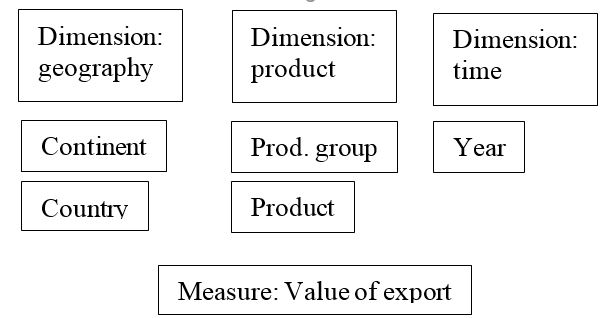
\includegraphics[scale=0.5]{fig1.JPG}
\caption{A visualization of a cube.\label{fig1}}
\end{figure}

As in our previous paper \cite{Nii181}, summarizability can be informally defined as
``correctness of aggregate data with respect to individual
observations''. In practice this is often implemented so that when a
user queries a cube, the query should be inspected in such a way that
the query's result cannot violate the conditions of summarizability. We
formulate the conditions as follows \cite{Tap14}: (i) The aggregation operation
(usually sum, mean or count) is appropriate for the measure and (ii) The
measure is appropriate for the aggregation levels in the cube's
dimensions.

We are specifically interested in

\begin{itemize}
\item
  the statistical scales of measure variables: nominal, ordinal,
  interval and ratio scales, since they affect which aggregation
  operation can be applied to the data
\item
  the ``eventness'' type of measure variable. These we classify as (i)
  tally measures that are intrinsic information about a specific event
  like quantity sold in sales data, (ii) reckoning measures like
  inventory levels and (iii) snapshot measures that are indirect
  measurement based on data at hand like currency exchange rates \cite{Tap14}.
\end{itemize}

Instead of checking the summarizability when evaluating a query, our
design (described in Section 3 below) aims at ensuring summariazablity
when the cube is constructed from data sets. This is not a definite
guarantee that all the user queries with the constructed cube will
result to ``correct'' answers. This is because in rare cases the
generated cube can contain multiple dimension-measure pairs (D\textsubscript{i}M\textsubscript{i}) such
that D\textsubscript{1}M\textsubscript{1} and
D\textsubscript{2}M\textsubscript{2} would ensure summarizability, but
the user manages formulate a query that returns an answer based on
D\textsubscript{1}M\textsubscript{2}. However, in the examples of this
paper, such a situation does not occur.

\subsection{The RDF Framework Description}\label{the-rdf-framework-description}

The amount of available data for business intelligence applications is
potentially very large and the data may have been stored in
geographically distributed manner, since it is profitable to run data
processing in a distributed way on demand. We have successfully applied
grid/cloud technologies for this purpose earlier \cite{Nii09}. Here, we define the
data sources using an ontology-based approach to map to original data
sources to an OLAP ontology describing a star schema. This approach
would also enable us to take advantage of common big data processing
platforms which usually offer a higher abstraction level, an efficient
distributed storage solution and greater computational power.

The applied methodology consists of the following steps:

1. Defining ontology descriptions for (big) data sources. These
descriptions contain definitions of data types with their summarizablity
information.

2. Retrieving the data based on the ontology descriptions. This step can
be performed in sequential and distributed fashion or applying
distributed query processing using a big data platform.

3. Collecting and aggregating the results of sub-queries, if the
previous step was distributed.

4. Creating the OLAP cube schema for the retrieved data and uploading
the data into user's analysis server (e.g. an OLAP tool or a statistical
software package).

In the first step, the available data is mapped into an OLAP ontology
using RDF \cite{Nie07}. This means identifying data sources, and their measure and
dimension attributes with their hierarchies. The ontology can also
contain information needed to guarantee the correctness of aggregations \cite{Tap14}.
In Steps 2 and 3, the data needed to answer the user's query at hand
is retrieved. Finally, in Step 4, the collected OLAP data is transformed
into a suitable format for uploading onto the analysis tool. This step
includes mapping the data types in the ontology into the data types used
in the analysis system.


\section{System Design and Implementation}

The goal of the design is to
provide a catalogue of data sets, combined with their meta data. The
users will upload data sets of their interest into the catalogue. After
each upload the catalogue software lets the user specify a description
of the data set. The data set is expected to have recognizable fields
that represent potential measures or (levels of) dimensions. For each
measure the user will record its statistical scale, ``eventness'' and
unit of measurement. For each dimension, the user will record its
description. An interface for entering the meta data after a file upload
are shown in Fig. \ref{fig2} and the uploaded data sets in Fig. \ref{fig3}.

\begin{figure}
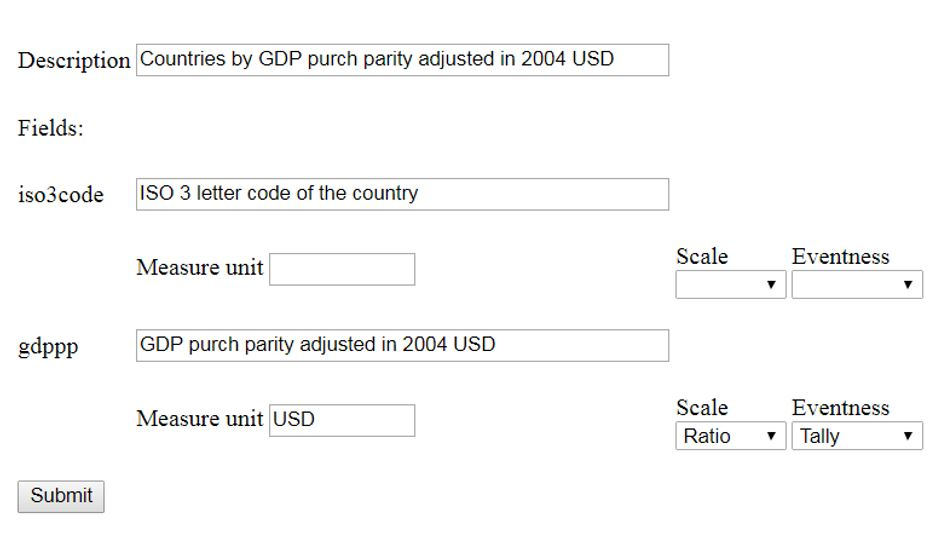
\includegraphics[scale=0.3]{fig2.JPG}
\caption{Meta-data editor.\label{fig2}}
\end{figure}

\begin{figure}
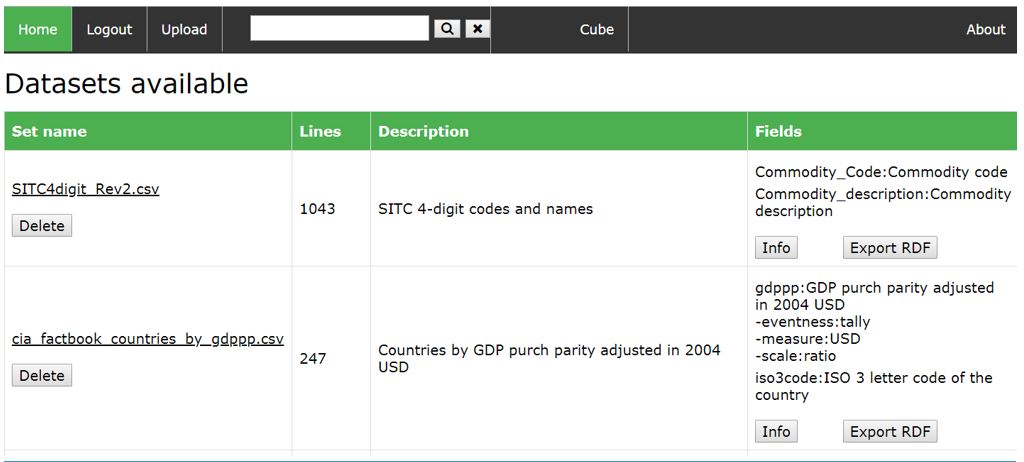
\includegraphics[scale=0.3]{fig3.JPG}
\caption{Uploaded data sets.\label{fig3}}
\end{figure}

Other than disk space, there is no limitation to the number of files
that can be managed by the platform. For clarity and brevity, however,
we assume that the files that the user has uploaded are those listed in
Table 1. Next, we shall demonstrate the process of selecting data sets,
combining them by measure and exporting the resulting cube to the R
statistics software.

The users starts the cube building by clicking on the Cube entry in the
menu of Fig. 3. The cube building process is iterative in such a way
that the users first select a pair of data sets and indicate the columns
by which the sets will be joined. The result of this operation is an
initial cube. The process continues so that the user selects more data
sets that are joined with initial cube. At each step the system
determines whether the integration is going to be successful. Figures
\ref{fig4}, \ref{fig5} and \ref{fig6} illustrate the process.

\begin{figure}
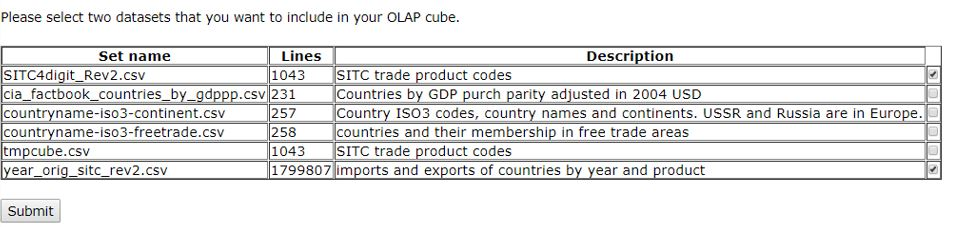
\includegraphics[scale=0.3]{fig4.JPG}
\caption{Cube building: selecting the data sets that will form the initial cube.\label{fig4}}
\end{figure}

\begin{figure}
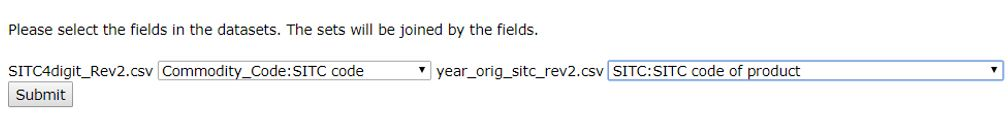
\includegraphics[scale=0.3]{fig5.JPG}
\caption{Cube building: selecting fields for the initial cube.\label{fig5}}
\end{figure}

\begin{figure}
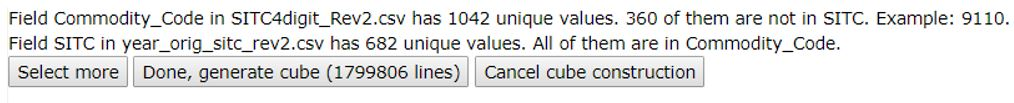
\includegraphics[scale=0.3]{fig6.JPG}
\caption{Cube building: analysis of selected fields.\label{fig6}}
\end{figure}

In Fig. 4, the user selects datasets ``year\_orig\_sitc\_rev2'' and
``SITC4digit\_rev2'' in order to map SITC4 trade codes to product names.
The process continues in Fig. 5 where the user selects the corresponding
columns. After this selection, the software analyses similarities of the
values of the fields as in Fig. 6.

As in our previous paper, we have tested the upload and download
performance of the dataspace application. Additionally, we can now
measure the performance of cube construction with R. The platform used
was an Intel Core i5 dual-core 2.4 GHz CPU computer with 4 GB RAM and a
normal 500 GB 7200 rpm disk. The dataspace application's upload speed is
ca 5MB/s and the download speed ca 38 MB/s. Reading and analyzing the
content of the CSV files in order to guarantee that the data can be
merged (see Fig. 6) is reasonably fast: our test computer was able to
read the data from the files, find the unique field values and compare
them at the speed of 330 000 lines per second. Writing the cube data
into a file is needed to provide the users with a CSV dataset that can
be loaded into a statistics package. The writing speed was about 150 000
lines per second.

With large files, memory management of the R software becomes
problematic. We tested reading speed with a file with 100 million
observations representing trade between countries for the years
2000..2016. Simply loading this data into R took 3 hours. In section 4
we discuss how to improve OLAP-style analysis for large data sets using
RDF.


\section{Distributed Analysis Using Hadoop}

There are several studies how to process RDF (SparQL) queries in Hadoop
\cite{Sch14}, \cite{Hus09} and \cite{Kaw16}, however, our OLAP approach makes it possible to use more a
straightforward and efficient approach. We divide the query processing
into two steps: 1) Data selection and preparation for roll-up
operations, 2) Aggregation computing. In the first step, we find the
required dimension attributes for each fact table row. For example, if
the resulting cube is requested to be on the `continent' level, we find
the corresponding continents for each country using the data in the
geography dimension. The dimension data is stored in HDFS and each
mapper process accesses it directly without using the mapreduce
protocol. This does not cause much overhead since dimension data is
usually small compared to fact table data. Instead, the fact table data
is distributed to the mappers in the normal mapreduce way. The data is
stored such a way that each row corresponds on OLAP fact row containing
the dimension keys and the measure values. In this way, each row is
independent so sending rows to different mappers does not cause
problems.

In this way, each reducer processes, i.e. aggregates, independent parts
of the data, so this can be done in parallel. In our example, data on
different continents can be process by different reducers. Finally, each
reducer writes it output and the final output, i.e. the requested OLAP
cube, is formed by combining these outputs. The MapReduce software was
implemented by using Python and it consists of the following parts:

Mapper:

\begin{enumerate}
\def\labelenumi{\arabic{enumi}.}
\item
  Initialise the RDF graph.
\item
  Read dimension data from HDFS and add it to the graph.
\item
  Read mapreduce input and add it to the graph.
\item
  Process a SparQL query for rolling up the dimension keys and selecting
  desired fact rows.
\item
  Serialize the query result and select a key. The key should be the
  most selective rolled-up dimension key to allow maximum parallelism in
  the reduce phase.
\end{enumerate}

\begin{quote}
Reducer:
\end{quote}

\begin{enumerate}
\def\labelenumi{\arabic{enumi}.}
\item
  Initialise the RDF graph.
\item
  Read mapreduce input from mappers and add it to the graph.
\item
  Process a SparQL query for aggregating the data.
\item
  Write the output
\end{enumerate}

We tested the method using a Hadoop cluster in an AWS cloud environment.
The mapper query was:

CONSTRUCT \{?continent aa:EXPORT\_VAL ?export\} WHERE \{?country
aa:Continent ?continent . ?country aa:ISO3digit ?iso . ?e\_id aa:ORIGIN
?iso . ?e\_id aa:EXPORT\_VAL ?export \}

and the reducer query:

CONSTRUCT \{?continent aa:EXPORT\_VAL ?exp\} WHERE \{ SELECT ?continent
(SUM(xsd:decimal(?export)) AS ?exp) WHERE \{?continent aa:EXPORT\_VAL
?export .\} GROUP BY ?continent \}.

The results are shown in Table 2. As we can see, adding more computing
nodes always decrease the computing time. However, improved performance
is not linear and also heavily depends on used node types. In practical
solutions, the gained performance improvements can be significant, since
using large enough clusters can trop the processing time less than a
tenth compared to the single node case.

\begin{table}[]
\begin{tabular}{lllll}
Type of       & Number      & Processing      & \% faster        & Times faster                        \\
nodes         & of slave    & time            & than one         & than one                            \\
              & nodes       & (real)          & ‘large‘ node     & ‘large’ node                        \\
\midrule
m4.large      & 1           & 64m 29.9s       &                  &                                     \\
m4.large      & 2           & 62m 48.8s       & 3\%              & 1.03                                \\
m4.large      & 4           & 29m 17.3s       & 55\%             & 2.2                                 \\
m4.large      & 8           & 14m 51.4s       & 77\%             & 4.34                                \\
m4.large      & 19          & 9m 25.1s        & 85\%             & 6.85                                \\
              &             &                 &                  & Times faster\\
              &             &                 &                  & than one\\
              &             &                 &                  & ‘xlarge’ node \\
m4.xlarge     & 1           & 33m 45.7s       & 48\%             &                                     \\
m4.xlarge     & 2           & 19m 56.7s       & 69\%             & 1.69                                \\
m4.xlarge     & 5           & 10m 31.7s       & 84\%             & 3.21                                \\
m4.xlarge     & 8           & 9m 9.5s         & 86\%             & 3.69                               \\
\end{tabular}
\caption{\label{table2}Hadoop processing}
\end{table}

In this paper we have presented a web-based dataspace management system
for large data sets. Our principal aim is to help data analysts discover
problems with data integration. This is done by storing the data sets
together with their meta data. The meta data includes scale,
``eventness'' and unit for measures and a list of compatible fields for
dimensions. The dataspace application supports an OLAP-like cube
construction into a file that can be used by statistics software. Our
test results indicate that using a distributed MapReduce framework in a
cloud computing cluster can decrease the processing time by 85\% or even
more depending on the number and type of the nodes in the cluster.

The web software was build using the Python Flask framework, available
for Microsoft Windows and other operating systems. The software is
freely available at
\url{https://sourceforge.net/projects/simple-dataspace-management}.

This research has been partially supported by Hasler Foundation (project
number 18039).

\bibliographystyle{plain}
\bibliography{niinimaki-opencs}

\end{document}
 
